\documentclass{article}
\usepackage{tikz}
\begin{document}

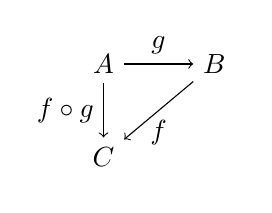
\begin{tikzpicture}[every node/.style={midway}]
\matrix[column sep={4em,between origins},
        row sep={2em}] at (0,0)
{ \node(A)   {$A$}  ; & \node(B) {$B$}; \\
  \node(C) {$C$};                   \\};
\draw[<-] (C) -- (A) node[anchor=east]  {$f\circ g$};
\draw[->] (B) -- (C) node[anchor=north]  {$f$};
\draw[->] (A)   -- (B) node[anchor=south] {$g$};
\end{tikzpicture}

\begin{Huge}
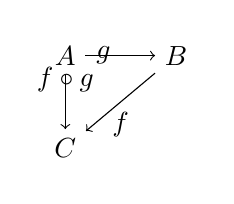
\begin{tikzpicture}[every node/.style={midway}]
\matrix[column sep={4em,between origins},
        row sep={2em}] at (0,0)
{ \node(A)   {$A$}  ; & \node(B) {$B$}; \\
  \node(C) {$C$};                   \\};
\draw[<-] (B) -- (A) node[anchor=east]  {$g$};
\draw[->] (B) -- (C) node[anchor=north]  {$f$};
\draw[->] (A) -- (C) node[anchor=south] {$f\circ g$};
\end{tikzpicture}
\end{Huge}

\end{document}